\qns{Transfer Function}

Create a Bode plot of the following transfer function:

$$H(\omega) = \frac{1}{10} \frac{((j\omega)^2 + 110j\omega + 1000)(j\omega + 10000)}
	{(j\omega+1000)((j\omega)^2 + 101j\omega + 100)}$$

\sol{

First of all, we decompose the second-order terms:
$$H(\omega) = \frac{1}{10} \frac{((j\omega)+100)(j\omega+10))(j\omega + 10000)}
	{(j\omega+1000)((j\omega)+100)(j\omega+1))}  =
		 \frac{1}{10} \frac{(j\omega+10)(j\omega + 10000)}
	{(j\omega+1000)(j\omega+1)}$$
Then, we convert it to the normal form:
$$H(\omega) =
		 \frac{10}{1} \frac{(\frac{j\omega}{10}+1)(\frac{j\omega}{10000} + 1)}
	{(\frac{j\omega}{1000}+1)(j\omega+1)}$$
	
\begin{figure}[H]
\centering
\scalebox{0.9}{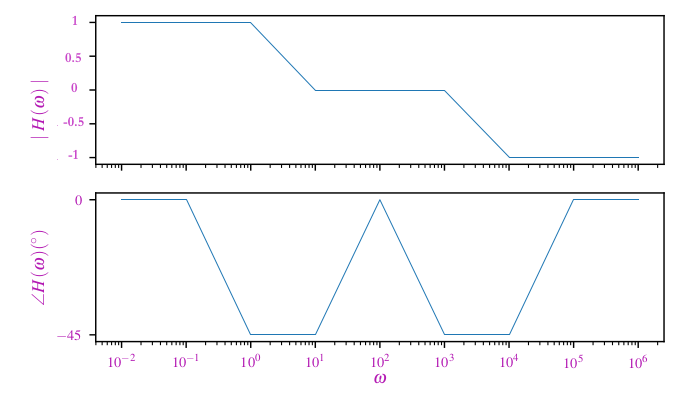
\includegraphics[scale=0.6]{\bank/transfer/figures/q_complicated_fixed.png}}
\end{figure}

}
